% !TeX program = xelatex
% !TeX encoding = UTF-8
% !TeX spellcheck = en_US
% !BIB program = biber
%% 
%% The above lines help editors like TeXstudio to automatically choose the right tools
%% to compile your LaTeX source file. If your tool does not support these magic comments,
%% you will need to make appropriate manual choices.
%% 
%% You can safely use "pdflatex" instead of "xelatex" if you prefer the pdfLaTeX toolchain.
%% However, pdfLaTeX will not be able to deliver the professional font experience that you
%% will get with XeLaTeX. You can also safely use "lualatex" instead of "xelatex" while
%% preserving the professional font experience if you prefer the LuaLaTeX toolchain.
%% 
%% _Important_: These magic comments should be on the first lines of your source file.
%% 
%%%%%%%%%%%%%%%%%%%%%%%%%%%%%%%%%%%%%%%%%%%%%%%%%%%%%%%%%%%%%%%%%%%%%%%%%%%%%%%%

%%%%%%%%%%%%%%%%%%%%%%%%%%%%%%%%%%%%%%%%%%%%%%%%%%%%%%%%%%%%%%%%%%%%%%%%%%%%%%%%
%% 
%%            JJJJ   K                         K   UUUU         UUUU  
%%            JJJJ   KKKK                   KKKK   UUUU         UUUU  
%%            JJJJ   KKKKKK               KKKKKK   UUUU         UUUU  
%%            JJJJ      KKKKKK         KKKKKK      UUUU         UUUU  
%%            JJJJ         KKKKKK   KKKKKK         UUUU         UUUU  
%%            JJJJ            KKKKKKKKK            UUUU         UUUU  
%%    JJ     JJJJJ               KKK               UUUUU       UUUUU  
%%  JJJJJJJJJJJJJ    KKKKKKKKKKKKKKKKKKKKKKKKKKK    UUUUUUUUUUUUUUU   
%%    JJJJJJJJJ      KKKKKKKKKKKKKKKKKKKKKKKKKKK      UUUUUUUUUUU     
%% 
%% This is an example file for using the JKU LaTeX Beamer Theme.
%% 
%% Template created by Susanne Hametner and Doris Pargfrieder
%% Template altered by Pieter-Jan Hoedt (2020)
%% Template rewritten by Michael Roland (2021)
%% 
%%%%%%%%%%%%%%%%%%%%%%%%%%%%%%%%%%%%%%%%%%%%%%%%%%%%%%%%%%%%%%%%%%%%%%%%%%%%%%%%

%%%%%%%%%%%%%%%%%%%%%%%%%%%%%%%%%%%%%%%%%%%%%%%%%%%%%%%%%%%%%%%%%%%%%%%%%%%%%%%%
%% 
%% Document class: This is a LaTeX beamer presentation.
%% 
\documentclass[utf8,aspectratio=169,ngerman,english]{beamer}
%% 
%% The comma-separated list in square brackets are class options.
%% Useful options that you might want to use:
%% 
%% Define the aspect ratio of the slide layout:
%%  * aspectratio=169  ... 16:9 aspect ratio
%%  * aspectratio=43   ... 4:3 aspect ratio
%%  * aspectratio=1610 ... 16:10 aspect ratio
%% 
%% Define document languages:
%%  * ngerman ... German
%%  * english ... English
%%  * ...
%% 
%% Note that adding multiple document languages allows you to switch between these languages
%% within the document (using e.g. the `otherlanguage' environment). The last language in
%% the class options will be used as the default document language.
%% 
%% Switch to handout mode:
%%  * handout ... A compact mode that allows you to remove animation and skips slides for
%%                efficient printing.
%% 
%% Other options:
%%  * utf8 ... Treat input files as UTF-8 encoded. Make sure to always provide that option
%%             when you use pdfLaTeX so that pdfLaTeX knows how to read and interpret
%%             characters in this source file.
%%  * c    ... Vertically center text on slides by default. You should avoid using this
%%             option. Only use this to restore the behavior of older versions of this theme.
%% 
%% _Important_: The document class should be the first line of LaTeX code in your main
%% source file. Do not place anything but comments / magic comments above that line (unless
%% you really know what you are doing).
%% 
%%%%%%%%%%%%%%%%%%%%%%%%%%%%%%%%%%%%%%%%%%%%%%%%%%%%%%%%%%%%%%%%%%%%%%%%%%%%%%%%

%%%%%%%%%%%%%%%%%%%%%%%%%%%%%%%%%%%%%%%%%%%%%%%%%%%%%%%%%%%%%%%%%%%%%%%%%%%%%%%%
%% 
%% Use the JKU LaTeX beamer theme for this presentation.
%% 
%\usetheme[TNF,nosectionpage]{jku}
\usetheme[darkmode,fancyfonts,totalframenumber,mathastext]{jku}
%% 
%% The comma-separated list in square brackets are theme options. Useful options that you
%% might want to use:
%% 
%% Color scheme selection options:
%%  * JKU  ... Use JKU (gray) color scheme (this is the default if no scheme is selected).
%%  * BUS  ... Use Business School color scheme.
%%  * LIT  ... Use Linz Institute of Technology color scheme.
%%  * MED  ... Use MED faculty color scheme.
%%  * RE   ... Use RE faculty color scheme.
%%  * SOE  ... Use School of Education color scheme.
%%  * SOWI ... Use SOWI faculty color scheme.
%%  * TNF  ... Use TNF faculty color scheme.
%% 
%% Color mode selection options:
%%  * darkmode ... Use dark color mode (where title and logo frames have a dark background).
%% 
%% Frame numbering options:
%%  * framenumber         ... Insert frame number into the frame footer.
%%  * totalframenumber    ... Insert frame number and total frame number into the frame footer
%%                            (only frames in the main part are counted).
%%  * appendixframenumber ... Similar to `totalframenumber', but count the overall total frame
%%                            number of main part and appendix.
%% 
%% Note that combining `totalframenumber' and `appendixframenumber' options will show the total
%% number of frames for the main part on frames in the main part and the overal total number of
%% frames for frames in the appendix.
%% 
%% Sectioning options:
%%  * nosectionpage       ... Supress section frames (see \section{<title>} command).
%%  * nosubsectionpage    ... Supress subsection frames (see \subsection{<title>} command).
%%  * nosubsubsectionpage ... Supress subsubsection frames (see \subsubsection{<title>} command).
%%  * partpage            ... Insert part frames (see \part{<title>} command).
%% 
%% Note that `nosectionpage' automatically sets `nosubsectionpage' and `nosubsubsectionpage'.
%% You could still e.g. show only subsubsection pages by using `nosectionpage,subsubsectionpage'.
%% 
%% Space-efficient monospace font options (requires XeTeX/LuaTeX):
%%  * compactmono   ... Use condensed fixed-width font everywhere.
%%  * nocompactverb ... Do not use condensed fixed-width font for verbatim and listings.
%% 
%% Style-breaking options:
%%  * nojkufooter    ... Do not insert JKU/partner logos into the frame footer.
%%  * nofooter       ... Do not display a frame footer.
%%  * noimprint      ... Do not insert imprint on title pages.
%%  * nojkulogo      ... Do not insert JKU & K logos on title pages and in frame footers.
%%  * frametitlecaps ... Set frame titles in capital letters (like in earlier theme versions).
%%  * nofancyfonts   ... Do not use custom TTF fonts with XeTeX/LuaTeX / supress pdfLaTeX warning.
%%  * mac            ... Use adapted color palette for screen display on Mac.
%%  * legacyitemizestyle ... Use old bullet style in itemization.
%% 
%% Advanced options:
%%  * mathastext        ... Use standard document fonts (enhanced with symbols from Fira Math
%%                          font when using XeTeX/LuaTeX) in math mode.
%%  * eulermath         ... Use Euler fonts in math mode with XeTeX/LuaTeX.
%%  * nooptpackages     ... Do not load additional convenience packages (which are only there
%%                          to provide interoperability to the behavior of previous versions of
%%                          this theme but are not actually required for the current version).
%%  * logopath={<path>} ... Set the path where the theme can find its own logo resources. This
%%                          should typically be a relative path and the default is `./logos'.
%%  * fontpath={<path>} ... Set the path where the theme can find its own font resources. This
%%                          should typically be a relative path and the default is `./fonts'.
%% 
%% Hint: Boolean options can be used in the forms `option' or `option=true' the enable the
%% option and `nooption' or `option=false' to disable the option.
%% 
%%%%%%%%%%%%%%%%%%%%%%%%%%%%%%%%%%%%%%%%%%%%%%%%%%%%%%%%%%%%%%%%%%%%%%%%%%%%%%%%

%%%%%%%%%%%%%%%%%%%%%%%%%%%%%%%%%%%%%%%%%%%%%%%%%%%%%%%%%%%%%%%%%%%%%%%%%%%%%%%%
%% 
%% This is the place where you can load additional packages. If you want to load
%% a package `booktabs', you would use the command `\usepackage{booktabs}'.
%% 

\usepackage{booktabs}
\usepackage{tabularx}
%\usepackage{pifont}
%\newcommand{\cmark}{\ding{51}}
%\newcommand{\xmark}{\ding{55}}
%\newcommand{\rarr}{\ding{212}}
%\newcommand{\larr}{\raisebox{\depth}{\rotatebox{180}{\rarr}}}
\usepackage{csquotes}
\usepackage[backend=biber,citestyle=authoryear,sortcites=true,style=ACM-Reference-Format]{biblatex}

%% 
%%%%%%%%%%%%%%%%%%%%%%%%%%%%%%%%%%%%%%%%%%%%%%%%%%%%%%%%%%%%%%%%%%%%%%%%%%%%%%%%

%%%%%%%%%%%%%%%%%%%%%%%%%%%%%%%%%%%%%%%%%%%%%%%%%%%%%%%%%%%%%%%%%%%%%%%%%%%%%%%%
%% 
%% Set reasonable defaults for biblatex.
%% 

\preto{\bibsetup}{\providecommand*{\insertbiblabel}{}}
\DeclareFieldFormat*{title}{#1}
\DeclareFieldFormat*{booktitle}{#1}
\DeclareFieldFormat*{journaltitle}{#1}
\setcounter{biburlnumpenalty}{100}
\setcounter{biburllcpenalty}{100}
\setcounter{biburlucpenalty}{100}

%% Add bibligraphy source files
\addbibresource{references.bib}

%% 
%%%%%%%%%%%%%%%%%%%%%%%%%%%%%%%%%%%%%%%%%%%%%%%%%%%%%%%%%%%%%%%%%%%%%%%%%%%%%%%%


\begin{document}

%%%%%%%%%%%%%%%%%%%%%%%%%%%%%%%%%%%%%%%%%%%%%%%%%%%%%%%%%%%%%%%%%%%%%%%%%%%%%%%%
%% 
%% Presentation information and title page
%% 

%% Command \series{series title}: sets the series title
%\series{Space for your lecure title}

%% Command \title[short title]{title}: sets the presentation title
%% Command \titlesmall{text}: switches to small font size inside title
\title{JKU Presentation Theme}

%% Command \subtitle[short subtitle]{subtitle}: sets the presentation subtitle
\subtitle{for \LaTeX\ Beamer}

%% Command \author[short authors]{authors}: sets the presentation authors (multiple authors may be separated with \and)
\author{Space for speaker names}

%% Command \institute{name}: sets the institute / author affiliation (style-breaking)
%\institute{Space for institute name}

%% Command \institutecode{CODE}: sets the institute abbreviation/initials (used to load the institute logo file, if present)
%\institutecode{INS}

%% Command \date[short date]{date}: sets the presentation date (short date is used in the footer by default)
%\date{\today}  % use this to set the date on the title page (style-breaking) and in the footer
\date[\today]{} % use this to set the date except for the title page (effectively in the footer only)

%% Command \partnerlogo[white=filename]{filename}: use filename as partner logo (leave filename blank to disable the partner logo), the optional argument ``white='' defines a separate file for use on dark background
%\partnerlogo{our_partner_logo}

%% Command \footer{text}: sets the footer field
%\footer{\insertsectionhead} % the default
%\footer{\insertshorttitle}  % a good alternative

%% Command \footerdate{text}: sets the footer date field
%\footerdate{\insertshortdate} % the default

%% Command \footerpartnerlogo{filename}: use a different partner logo in the footer (e.g. a logo with a different form factor or no filename to disable the partner logo in the footer)
%\footerpartnerlogo{our_partner_logo}

%% Command \agenda[caption]{text}: sets the agenda (and optional caption) to display on the next title or section page
%\agenda[caption]{text}


%% Finally, print the title page using the above information:
%% 
%% \maketitle[options]
%%     Inserts a title page. The current standard faculty color theme and color
%%     mode are used by default, you may modify this using any of the following
%%     options:
%%      * light ... use light color theme
%%      * dark  ... use dark color theme
%%      * gray  ... use JKU gray color theme
%%      * black ... use black background
%%     In addition, options may contain a faculty name (see theme options) to
%%     use the faculty's color theme, e.g. `\maketitle[LIT,dark]'.
%% 
\maketitle
%% 
%% Note that you can even change the presentation information and print another
%% title page (with that updated information) ANYWHERE in your presentation.
%% 
%%%%%%%%%%%%%%%%%%%%%%%%%%%%%%%%%%%%%%%%%%%%%%%%%%%%%%%%%%%%%%%%%%%%%%%%%%%%%%%%


%% 
%% You can split your presentation into sections, subsections, and subsubsections,
%% just like you would do with any other LaTeX document. Depending on the chosen
%% theme options, frames showing the section titles will be inserted for each
%% sectioning command. You can use the starred versions of these commands (e.g.
%% `\section*{<title>}') to suppress specific section title frames.
%% 
\section{Prerequisites}

%% 
%% You create a new slide using the `frame' environment:
%% 
\begin{frame}
\frametitle{Installation}

\begin{itemize}
\item Download the latest version of the theme package from \url{https://github.com/michaelroland/jku-templates-presentation-latex}.
\item Extract its contents (unzip) and move the files to a location on your computer where {\LaTeX} will find them. The most portable choice is the folder of your main presentation file.
\item Use \texttt{main.tex} (the source of this presentation) as a starting point for building your own presentation. It contains detailed guides about the various package options.
\item Use \texttt{xelatex} or \texttt{lualatex} as the {\LaTeX} typesetting engine (because they include enhanced font support). \texttt{pdflatex} is also supported but does not deliver the full theme experience.
\end{itemize}
\end{frame}


\begin{frame}
\frametitle{Theme Package Requirements}

This theme requires that the following packages are installed:
\begin{columns}[onlytextwidth]
\column{0.4\textwidth}
\begin{itemize}
\item \texttt{amsmath}
\item \texttt{babel}
\item \texttt{beamer}
\item \texttt{datetime2}
\item \texttt{etoolbox}
\item \texttt{fontawesome5}
\item \texttt{fontspec} (only with XeTeX/LuaLaTeX)
\end{itemize}

\column{0.4\textwidth}
\begin{itemize}
\item \texttt{hyperref}
\item \texttt{iftex}
\item \texttt{inconsolata}
\item \texttt{listings}
\item \texttt{lm}
\item \texttt{pgf}
\item \texttt{psnfss}
\item \texttt{translations}
\end{itemize}

\column{0.2\textwidth}
\begin{itemize}
\item \texttt{xkeyval}
\item \texttt{xcolor}
\end{itemize}
\end{columns}
\end{frame}


\section{Getting Started}

\begin{frame}[containsverbatim]
\frametitle{Getting Started}

\begin{itemize}
\item Begin your new presentation with \verb|\documentclass[<class options>]{beamer}|, where \verb|<class options>| is a comma-separated list of options:
    \begin{itemize}
    \item A typical class option is \verb|aspectratio=169| to set the slide aspect ratio to 16:9. Use \verb|aspectratio=43| to set the slide aspect ratio to 4:3.
    \item You should define at least one document language, e.g.\ \verb|english| or \verb|ngerman| (the ``n'' is intended). The last language will become the document default language.
    \item When you use pdfLaTeX, always add the option \verb|utf8| so that input files are treated as UTF-8 encoded.
    \end{itemize}

\item Next, select the JKU beamer theme with \verb|\usetheme[<theme options>]{jku}| (\verb|<theme options>| is, again, a comma-separated list of options).
\end{itemize}
\end{frame}


\subsection{Theme Options}

\begin{frame}[containsverbatim,label={options:colorscheme}]
\frametitle{Theme Options: Selecting a Color Scheme}
%\begin{table}
    \begin{tabularx}{\linewidth}{ll>{\raggedright}X}
    \toprule
    \textbf{Option} & \textbf{Color Scheme} & \textbf{Primary Color} \tabularnewline
    \midrule
    \textverb{JKU}    & JKU (gray) scheme                   & \mbox{\usebeamercolor[fg]{palette jku}\rule{6em}{10pt}} \tabularnewline
    \textverb{BUS}    & Business School scheme              & \mbox{\usebeamercolor[fg]{palette bus}\rule{6em}{10pt}} \tabularnewline
    \textverb{LIT}    & Linz Institute of Technology scheme & \mbox{\usebeamercolor[fg]{palette lit}\rule{6em}{10pt}} \tabularnewline
    \textverb{MED}    & MED faculty scheme                  & \mbox{\usebeamercolor[fg]{palette med}\rule{6em}{10pt}} \tabularnewline
    \textverb{RE}     & RE faculty scheme                   & \mbox{\usebeamercolor[fg]{palette re}\rule{6em}{10pt}} \tabularnewline
    \textverb{SOE}    & School of Education scheme          & \mbox{\usebeamercolor[fg]{palette soe}\rule{6em}{10pt}} \tabularnewline
    \textverb{SOWI}   & SOWI faculty scheme                 & \mbox{\usebeamercolor[fg]{palette sowi}\rule{6em}{10pt}} \tabularnewline
    \textverb{TNF}    & TNF faculty scheme                  & \mbox{\usebeamercolor[fg]{palette tnf}\rule{6em}{10pt}} \tabularnewline
    \bottomrule
    \end{tabularx}
%\end{table}

\smallskip
If no color scheme option is given, the package defaults to using \texttt{JKU}.
\end{frame}


\begin{frame}[containsverbatim,label={options:colormode}]
\frametitle{Theme Options: Selecting a Color Mode}
\begin{itemize}
\item The theme uses light color mode by default. In this color mode, all frames (including title, logo, and section frames) have a white background.
\item Use option ``\verb|darkmode|'' to display title, logo, and section frames with a dark background (primary color of the current color scheme).
\end{itemize}
\end{frame}


\begin{frame}[containsverbatim,label={options:slide-numbers}]
\frametitle{Theme Options: Slide Numbers}
No slide numbers are shown in slide footers by default. Enable them with:

\smallskip
%\begin{table}
    \begin{tabularx}{\linewidth}{l>{\raggedright}X}
    \toprule
    \textbf{Option}                & \textbf{Description} \tabularnewline
    \midrule
    \textverb{framenumber}         & Insert slide number into the footer. \tabularnewline
    \textverb{totalframenumber}    & Insert slide number and total slide number into the footer. \tabularnewline
    \textverb{appendixframenumber} & Like ``\textverb{totalframenumber}'', but also count slides from the appendix into the total. Combine with ``\textverb{totalframenumber}'' to only show the overall total for appendix slides. \tabularnewline
    \bottomrule
    \end{tabularx}
%\end{table}

\smallskip
Btw., if you want to reference a slide number, use the option \verb+[label={s}]+ in the target frame. Then \verb+\ref{s}+ will give a reference to the slide number. For instance, slide~\ref{options:section-slides} is the next slide.
\end{frame}


\begin{frame}[containsverbatim,label={options:section-slides}]
\frametitle{Theme Options: Section Slides}
By default, each sectioning command (\verb|\section|, \verb|\subsection|, \verb|\subsubsection|) inserts a section slide. You can globally disable section slides with:

\smallskip
%\begin{table}
    \begin{tabularx}{\linewidth}{l>{\raggedright}X}
    \toprule
    \textbf{Option}            & \textbf{Description} \tabularnewline
    \midrule
    \textverb{nosectionpage}       & Supress all section slides. \tabularnewline
    \textverb{nosubsectionpage}    & Supress subsection and subsubsection slides. \tabularnewline
    \textverb{nosubsubsectionpage} & Supress subsubsection slides. \tabularnewline
    \bottomrule
    \end{tabularx}
%\end{table}

\smallskip
\begin{itemize}
\item The class option \verb|handout| also supresses these slides but includes them in slide numbering.
\item The starred versions of sectioning commands (e.g.\ \verb|\section*{...}|) also supress section slides. 
\end{itemize}
\end{frame}


\begin{frame}[containsverbatim]
\frametitle{More Theme Options}
%\begin{table}
    \begin{tabularx}{\linewidth}{l>{\raggedright}X}
    \toprule
    \textbf{Option}			     & \textbf{Description} \tabularnewline
    \midrule
    \textverb{compactmono}         & Use condensed fixed-width font everywhere. \tabularnewline
    \textverb{nocompactverb}       & Do not use condensed fixed-width font for verbatim and listings. \tabularnewline
    \textverb{nofooter}            & Supress slide footer. \tabularnewline
    \textverb{nojkufooter}         & Supress JKU/partner logos in slide footer. \tabularnewline
    \textverb{noimprint}           & Supress imprint on title slides. \tabularnewline
    \textverb{nooptpackages}       & Do not load additional convenience packages (which are only there to provide interoperability to the behavior of previous versions of this theme but are not actually required for the current version). \tabularnewline
    \bottomrule
    \end{tabularx}
%\end{table}
\end{frame}


\subsection{Title Slide \& Slide Footers}

\begin{frame}[containsverbatim]
\frametitle{Title Slide}

Use \verb+\maketitle+ to display a title slide. This command uses the following information:

\smallskip
%\begin{table}
    \begin{tabularx}{\linewidth}{l>{\raggedright}X}
    \toprule
    \textbf{Command}                    & \textbf{Description} \tabularnewline
    \midrule
    \textverb{\string\title\{...\}}     & The title of your presentation. \tabularnewline
    \textverb{\string\subtitle\{...\}}  & The subtitle of your presentation. \tabularnewline
    \textverb{\string\author\{...\}}    & The speakers / authors of the presentation.
                                          % Use \textverb{\string\and} to separate multiple author names. 
                                          \tabularnewline
    \textverb{\string\institute\{...\}} & The intitute / affiliations of the author(s). \tabularnewline
    \textverb{\string\date\{...\}}      & The date of the presentation. Defaults to today's date if omitted. Use \textverb{\string\date\{\}} to supress the date. \tabularnewline
    \bottomrule
    \end{tabularx}
%\end{table}

\smallskip
\small An optional argument (\verb|\cmd[opt]{...}|) allows to set short versions for use in e.g.\ footers.
\end{frame}


\begin{frame}[containsverbatim,label={advanced-title-slides}]
\frametitle{Advanced Title Slides}

\begin{itemize}
\item You can change the presentation information and use the \verb+\maketitle+ command multiple times in your presentation.
\item An optional argument \verb|\maketitle[<options>]| allows to change the color scheme of the title slide. Options may be one of:
    \begin{itemize}
    \item \textverb{light}: Use light color theme.
    \item \textverb{dark}: Use dark color theme.
    \item \textverb{gray}: Use JKU gray color theme.
    \item \textverb{black}: Use black background.
    \end{itemize}
    In addition, options may contain a faculty name (see \hyperref[options:colorscheme]{Theme Options: Selecting a Color Scheme}) to use the faculty's color theme, e.g. ``\verb|\maketitle[TNF,dark]|''.
\end{itemize}
\end{frame}

\title{Space for new title}
\subtitle{Space for new subtitle}
\maketitle[TNF,dark]


\begin{frame}[containsverbatim]
\frametitle{Logos}

%\begin{table}
    \begin{tabularx}{\linewidth}{l>{\raggedright}X}
    \toprule
    \textbf{Command}                           & \textbf{Description} \tabularnewline
    \midrule
    \textverb{\string\institutecode\{code\}}   & The abbreviation / initials of the institute. Use this to load your institute logo instead of the standard JKU logo. E.g.\ \textverb{\string\institutecode\{LIT\}} to load the LIT logo. You need to add your logo files to the logos folder. \tabularnewline
    \textverb{\string\partnerlogo\{filename\}} & The logo of a partner institution. \textverb{filename} must point to an image file. File extension may be omitted. \tabularnewline
    \textverb{\string\footerpartnerlogo\{...\}} & Change the partner logo in the footer. Use this only if you need to display a different partner logo file (e.g.\ with a different geometry) in the footer. \tabularnewline
    \bottomrule
    \end{tabularx}
%\end{table}
\end{frame}


\begin{frame}[containsverbatim]
\frametitle{Customizing the Slide Footer}

%\begin{table}
    \begin{tabularx}{\linewidth}{l>{\raggedright}X}
    \toprule
    \textbf{Command}                                 & \textbf{Description} \tabularnewline
    \midrule
    \textverb{\string\footer\{...\}}                 & Use a customized footer text (defaults to the current section title). Use \textverb{\string\footer\{\string\insertshorttitle\}} to display the (short) presentation title instead. \tabularnewline
    \textverb{\string\footerdate\{...\}}             & Use a customized date field in the footer (defaults to \textverb{\string\footerdate\{\string\insertshortdate\}}). \tabularnewline
    \bottomrule
    \end{tabularx}
%\end{table}
\end{frame}


\subsection{Basic Elements}


\begin{frame}[containsverbatim]
\frametitle{Frames}

A slides is called \verb|frame| in \LaTeX\ beamer. It consists of a frame title and a body:
\begin{lstlisting}[language={[LaTeX]TeX},numbers=none]
\begin{frame}
\frametitle{Space for your frame title.}

Space for your frame body.
\end{frame}
\end{lstlisting}
\end{frame}


\begin{frame}[containsverbatim]
\frametitle{Bullet Items}

\begin{columns}[onlytextwidth,T]

\column{.5\textwidth}
\begin{itemize}
\item Item 1
    \begin{itemize}
    \item Subitem 1
        \begin{itemize}
        \item Subsubitem 1
        \end{itemize}
    \end{itemize}
\item Item 2
    \begin{itemize}
    \item Subitem 2
        \begin{itemize}
        \item Only three levels of nesting are supported ...~and this is good!
        \end{itemize}
    \end{itemize}
\end{itemize}

\column{.5\textwidth}
\begin{lstlisting}[language={[LaTeX]TeX},numbers=none]
\begin{itemize}
\item Item 1
    \begin{itemize}
    \item Subitem 1
        \begin{itemize}
        \item Subsubitem 1
        \end{itemize}
    \end{itemize}
\item Item 2
    \begin{itemize}
    \item Subitem 2
    \end{itemize}
\end{itemize} 
\end{lstlisting}

\end{columns}
\end{frame}


\begin{frame}[containsverbatim]
\frametitle{Enumerations}

\begin{columns}[onlytextwidth,T]

\column{.5\textwidth}
\begin{enumerate}
\item Item 1
    \begin{enumerate}
    \item Subitem 1
        \begin{enumerate}
        \item Subsubitem 1
        \end{enumerate}
    \end{enumerate}
\item Item 2
    \begin{enumerate}
    \item Subitem 2
    \end{enumerate}
\end{enumerate}

\column{.5\textwidth}
\begin{lstlisting}[language={[LaTeX]TeX},numbers=none]
\begin{enumerate}
\item Item 1
    \begin{enumerate}
    \item Subitem 1
        \begin{enumerate}
        \item Subsubitem 1
        \end{enumerate}
    \end{enumerate}
\item Item 2
    \begin{enumerate}
    \item Subitem 2
    \end{enumerate}
\end{enumerate} 
\end{lstlisting}

\end{columns}
\end{frame}


\begin{frame}[containsverbatim]
\frametitle{Columns}

\begin{columns}[onlytextwidth,T]

\column{.45\textwidth}
Use the columns environment to split the frame body into multiple columns:
\begin{lstlisting}[language={[LaTeX]TeX},numbers=none]
\begin{columns}[onlytextwidth,T]
...
\end{columns}
\end{lstlisting}
The options ``\textverb{onlytextwidth,T}'' are sensible defaults to make columns span only the normal text width of the slide and to vertically align column contents to the top.

\column{.50\textwidth}
Begin a new column with \verb|\column{<width>}|. You can use e.g.\ \verb|\column{.45\textwidth}| to let a column span 45\,\% of the normal text width.
\begin{lstlisting}[language={[LaTeX]TeX},numbers=none]
\begin{columns}[onlytextwidth,T]
\column{.45\textwidth}
Space for column 1.

\column{.50\textwidth}
Space for column 2.
\end{columns}
\end{lstlisting}

\end{columns}
\end{frame}


\begin{frame}[fragile]
\frametitle{Conditionally Reveal Items}

\begin{itemize}
\item A frame can actually span across multiple pages of your presentation to emulate ``appear'' animations.
\pause
\item Use the \textverb{\string\pause} command to reveal content.
\end{itemize}

\bigskip
\begin{lstlisting}[language={[LaTeX]TeX},numbers=none]
\begin{itemize}
\item A frame can actually span across multiple pages of your presentation to ...
\pause
\item Use the \textverb{\string\pause} command to reveal content.
\end{itemize}
\end{lstlisting}
\end{frame}


\begin{frame}[containsverbatim]
\frametitle{Table of Contents}

Use the \verb|\tableofcontents| command to list all sections and subsections in the presentation (if you really want to do this~\cite{schultz}):

\medskip
\tableofcontents
\end{frame}


\begin{frame}[containsverbatim]
\frametitle{Table of Contents: Keep it Compact}

Use the \verb|hideallsubsections| option to keep the table of contents more compact by including only first-level sections:

\medskip
\tableofcontents[hideallsubsections]

\bigskip
\begin{lstlisting}[language={[LaTeX]TeX},numbers=none]
\begin{frame}
\frametitle{Table of Contents}
\tableofcontents[hideallsubsections]
\end{frame}
\end{lstlisting}
\end{frame}


\begin{frame}[containsverbatim]
\frametitle{Blocks}

\begin{block}{Standard Block}
Content can be highlighted in so-called blocks. This is a standard \textverb{block}.
\end{block}

\begin{lstlisting}[language={[LaTeX]TeX},numbers=none]
\begin{block}{Space for title.}
Space for content.
\end{block} 
\end{lstlisting}
\end{frame}


\begin{frame}[containsverbatim]
\frametitle{Colorful Blocks}

\begin{alertblock}{Alert Block}
This is an \textverb{alertblock}.
\end{alertblock}
\vspace*{-.25ex}
\begin{lstlisting}[language={[LaTeX]TeX},numbers=none]
\begin{alertblock}{Space for title.}
Space for content.
\end{alertblock} 
\end{lstlisting}

\begin{exampleblock}{Example Block}
This is an \textverb{exampleblock}.
\end{exampleblock}
\vspace*{-.25ex}
\begin{lstlisting}[language={[LaTeX]TeX},numbers=none]
\begin{exampleblock}{Space for title.}
Space for content.
\end{exampleblock} 
\end{lstlisting}
\end{frame}


\begin{frame}[containsverbatim]
\frametitle{Lists with Reduced Spacing}

In some rare situations, it may be useful to create lists with reduced vertical spacing. Use the \verb|tightlist| environment for this:

\begin{columns}[onlytextwidth,T]

\column{.5\textwidth}
\begin{tightlist}
    \begin{itemize}
    \item Item 1
    \item Item 2
    \item Item 3
    \end{itemize}
\end{tightlist}

\column{.5\textwidth}
\begin{itemize}
\item Item 1
\item Item 2
\item Item 3
\end{itemize}

\end{columns}

\bigskip
\begin{columns}[onlytextwidth,T]

\column{.5\textwidth}
\begin{lstlisting}[language={[LaTeX]TeX},numbers=none]
\begin{tightlist}
    \begin{itemize}
    \item Item 1
    \item Item 2
    \item Item 3
    \end{itemize}
\end{tightlist}
\end{lstlisting}

\column{.5\textwidth}
\begin{lstlisting}[language={[LaTeX]TeX},numbers=none]
\begin{itemize}
\item Item 1
\item Item 2
\item Item 3
\end{itemize}
\end{lstlisting}

\end{columns}
\end{frame}


\section{Colors}

\begin{frame}
\frametitle{Color in Presentation}

\begin{itemize}
\item Consider the ``\textverb{darkmode}'' theme option in combination with one of the faculty-specific color schemes (see slides~\ref{options:colorscheme} \& \ref{options:colormode}) to add decent coloring to your presentation.
\item If you need colors in your presentation, use one of the pre-defined JKU colors.
\item Use \textverb{\string\textcolor\{<color>\}\{<text>\}} to display colored text.
\item Mac-users may want to use the theme option ``\textverb{mac}'' (for screen display versions of your presentation only!)
\end{itemize}
\end{frame}


\begin{frame}
\frametitle{JKU Colors}

\begin{columns}[onlytextwidth,T]

\column{0.20\textwidth}
\setbeamercolor{thisboxcolor}{bg=jkuBlue,fg=white}
\begin{beamercolorbox}[wd=\linewidth,ht=4ex,dp=2.5ex]{thisboxcolor}
\centering
\textverb{jkuBlue}
\end{beamercolorbox}

\vspace{2em}
\setbeamercolor{thisboxcolor}{bg=jkuCyan,fg=black}
\begin{beamercolorbox}[wd=\linewidth,ht=4ex,dp=2.5ex]{thisboxcolor}
\centering
\textverb{jkuCyan}
\end{beamercolorbox}

\vspace{2em}
\setbeamercolor{thisboxcolor}{bg=black,fg=white}
\begin{beamercolorbox}[wd=\linewidth,ht=4ex,dp=2.5ex]{thisboxcolor}
\centering
\textverb{black}
\end{beamercolorbox}


\column{0.20\textwidth}
\setbeamercolor{thisboxcolor}{bg=jkuYellow,fg=black}
\begin{beamercolorbox}[wd=\linewidth,ht=4ex,dp=2.5ex]{thisboxcolor}
\centering
\textverb{jkuYellow}
\end{beamercolorbox}

\vspace{2em}
\setbeamercolor{thisboxcolor}{bg=jkuGrey,fg=white}
\begin{beamercolorbox}[wd=\linewidth,ht=4ex,dp=2.5ex]{thisboxcolor}
\centering
\textverb{jkuGrey}
\end{beamercolorbox}

\vspace{2em}
\setbeamercolor{thisboxcolor}{bg=white,fg=black}
\begingroup
\setlength\fboxsep{0pt}
\fbox{\begin{beamercolorbox}[wd=\linewidth,ht=4ex,dp=2.5ex]{thisboxcolor}
\centering
\textverb{white}
\end{beamercolorbox}}
\endgroup

\column{0.20\textwidth}
\setbeamercolor{thisboxcolor}{bg=jkuLightGreen,fg=black}
\begin{beamercolorbox}[wd=\linewidth,ht=4ex,dp=2.5ex]{thisboxcolor}
\centering
\textverb{jkuLightGreen}
\end{beamercolorbox}

\vspace{2em}
\setbeamercolor{thisboxcolor}{bg=jkuGreen,fg=black}
\begin{beamercolorbox}[wd=\linewidth,ht=4ex,dp=2.5ex]{thisboxcolor}
\centering
\textverb{jkuGreen}
\end{beamercolorbox}


\column{0.20\textwidth}
\setbeamercolor{thisboxcolor}{bg=jkuPurple,fg=white}
\begin{beamercolorbox}[wd=\linewidth,ht=4ex,dp=2.5ex]{thisboxcolor}
\centering
\textverb{jkuPurple}
\end{beamercolorbox}

\vspace{2em}
\setbeamercolor{thisboxcolor}{bg=jkuRed,fg=white}
\begin{beamercolorbox}[wd=\linewidth,ht=4ex,dp=2.5ex]{thisboxcolor}
\centering
\textverb{jkuRed}
\end{beamercolorbox}

\end{columns}
\end{frame}


\section{Special Frames}

\begin{frame}[containsverbatim,plain]
\frametitle{Plain Frames}

The frame environment also takes optional arguments \verb|\begin{frame}[<options>]|. You already read about the ``\verb|label=|'' option on slide~\ref{options:slide-numbers}. Another option is \verb|plain| to supress the footer for a frame.

\begin{lstlisting}[language={[LaTeX]TeX},numbers=none]
\begin{frame}[plain]
\frametitle{Space for your frame title.}

Space for your frame body.
\end{frame}
\end{lstlisting}
\end{frame}


\begin{frame}[containsverbatim,plain]
Omit the frame title to get an empty frame.

\begin{lstlisting}[language={[LaTeX]TeX},numbers=none]
\begin{frame}[plain]
Space for your frame body.
\end{frame}
\end{lstlisting}
\end{frame}


\begingroup
\setbeamercolor{background canvas}{bg=jkuYellow}
\setbeamercolor{normal text}{fg=white}
\usebeamercolor[fg]{normal text}
\begin{frame}[containsverbatim]
\frametitle{Colorful Background}

You can change the background color of a frame by changing the color ``\textverb{background canvas}''. The standard foreground color is ``\textverb{normal text}''.

\color{black}
\begin{lstlisting}[language={[LaTeX]TeX},numbers=none]
\begingroup
\setbeamercolor{background canvas}{bg=jkuYellow}
\setbeamercolor{normal text}{fg=white}
\usebeamercolor[fg]{normal text}
\begin{frame}[plain]
\frametitle{Space for your frame title.}

Space for your frame body.
\end{frame}
\endgroup
\end{lstlisting}
\end{frame}
\endgroup


\begingroup
\usebackgroundtemplate{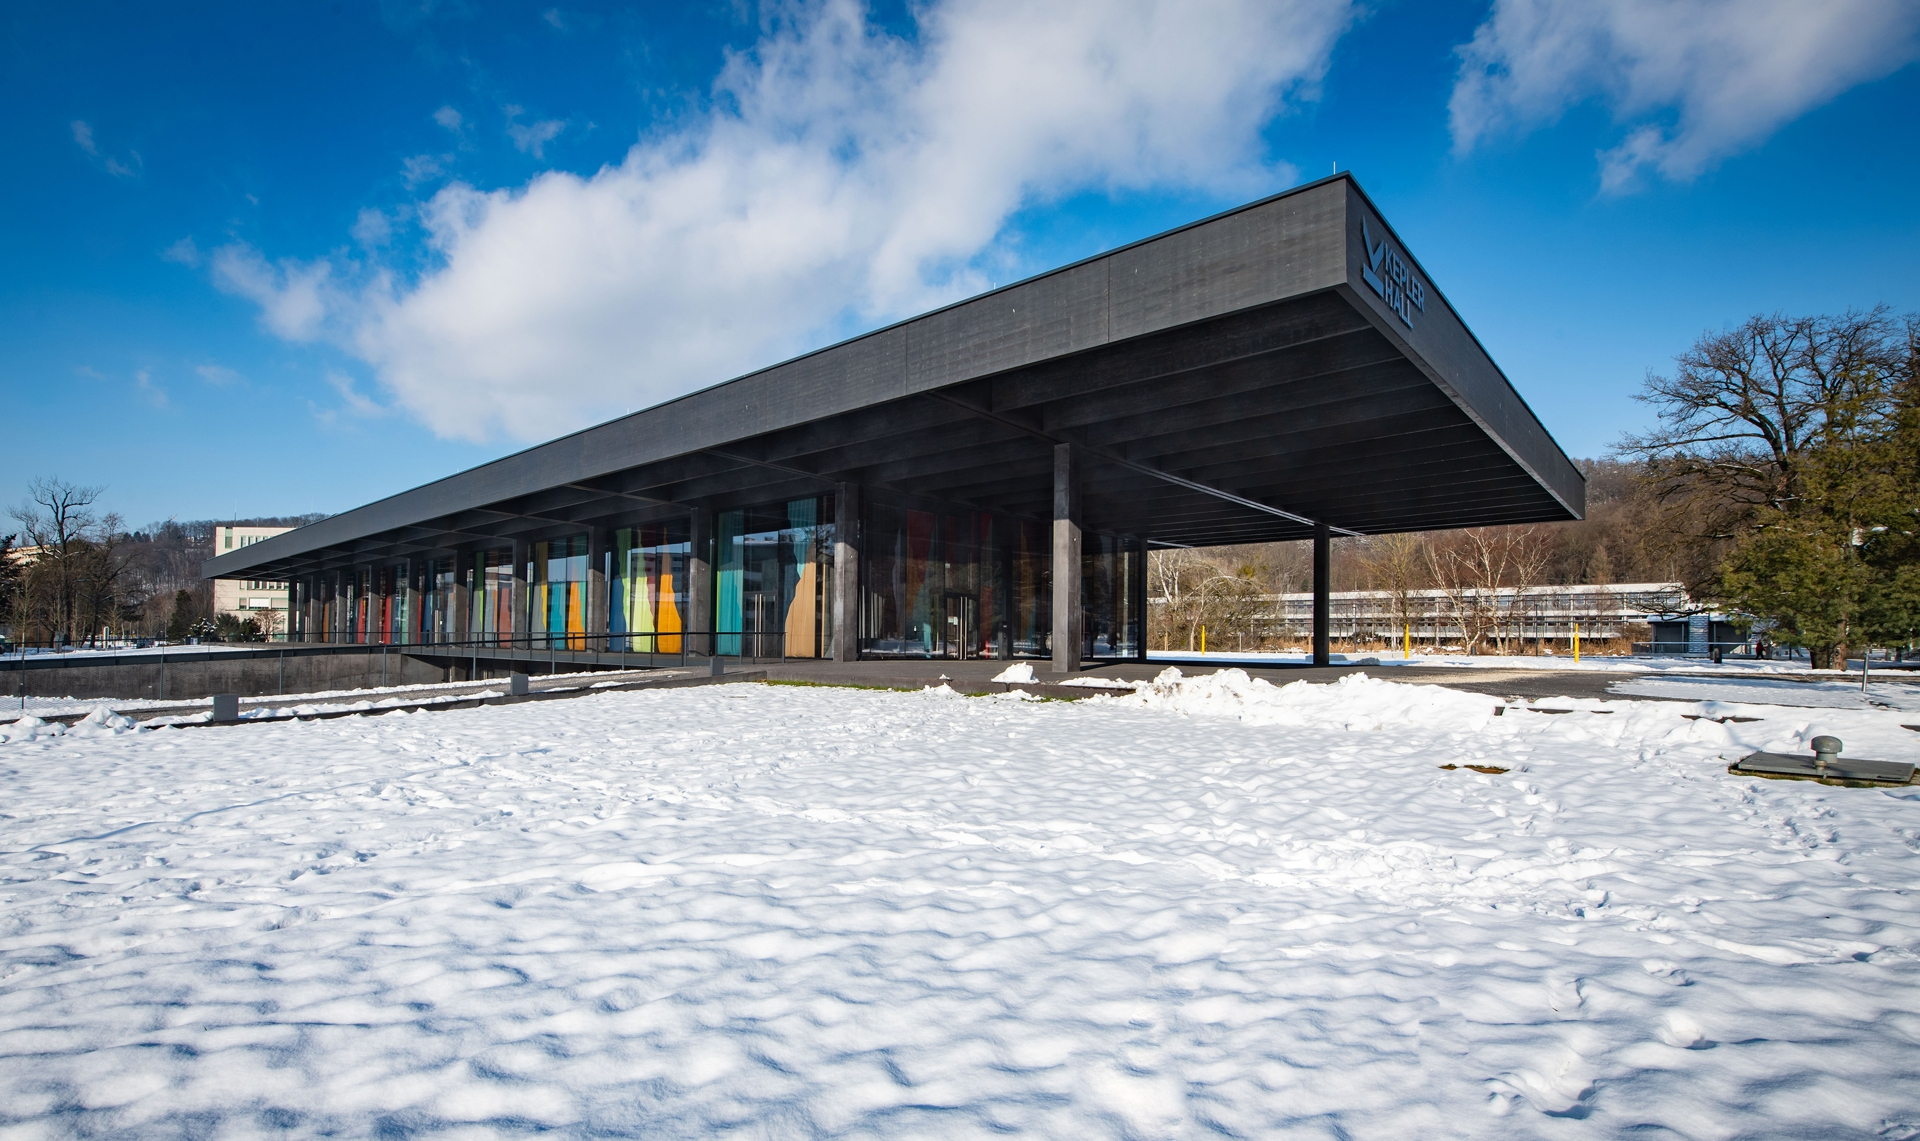
\includegraphics[width=\paperwidth]{images/jku_keplerhall_winter.jpg}}
\setbeamercolor{normal text}{fg=white}
\usebeamercolor[fg]{normal text}
\begin{frame}[containsverbatim,plain]
\frametitle{Background Image}

You can add a full screen background image to a slide. The aspect ratio of the picture should match the presentation. To fill the whole screen you might use \verb|height=\paperheight|, but the result might be distorted~\ldots

\bigskip
\setbeamercolor{thisboxcolor}{bg=white,fg=black}
\pgfsetfillopacity{0.6}
\begin{beamercolorbox}[wd=\linewidth,dp=0ex,vmode]{thisboxcolor}
\pgfsetfillopacity{1.0}
\begin{lstlisting}[language={[LaTeX]TeX},numbers=none,xleftmargin=0.5em,xrightmargin=0.5em]
\begingroup
\usebackgroundtemplate{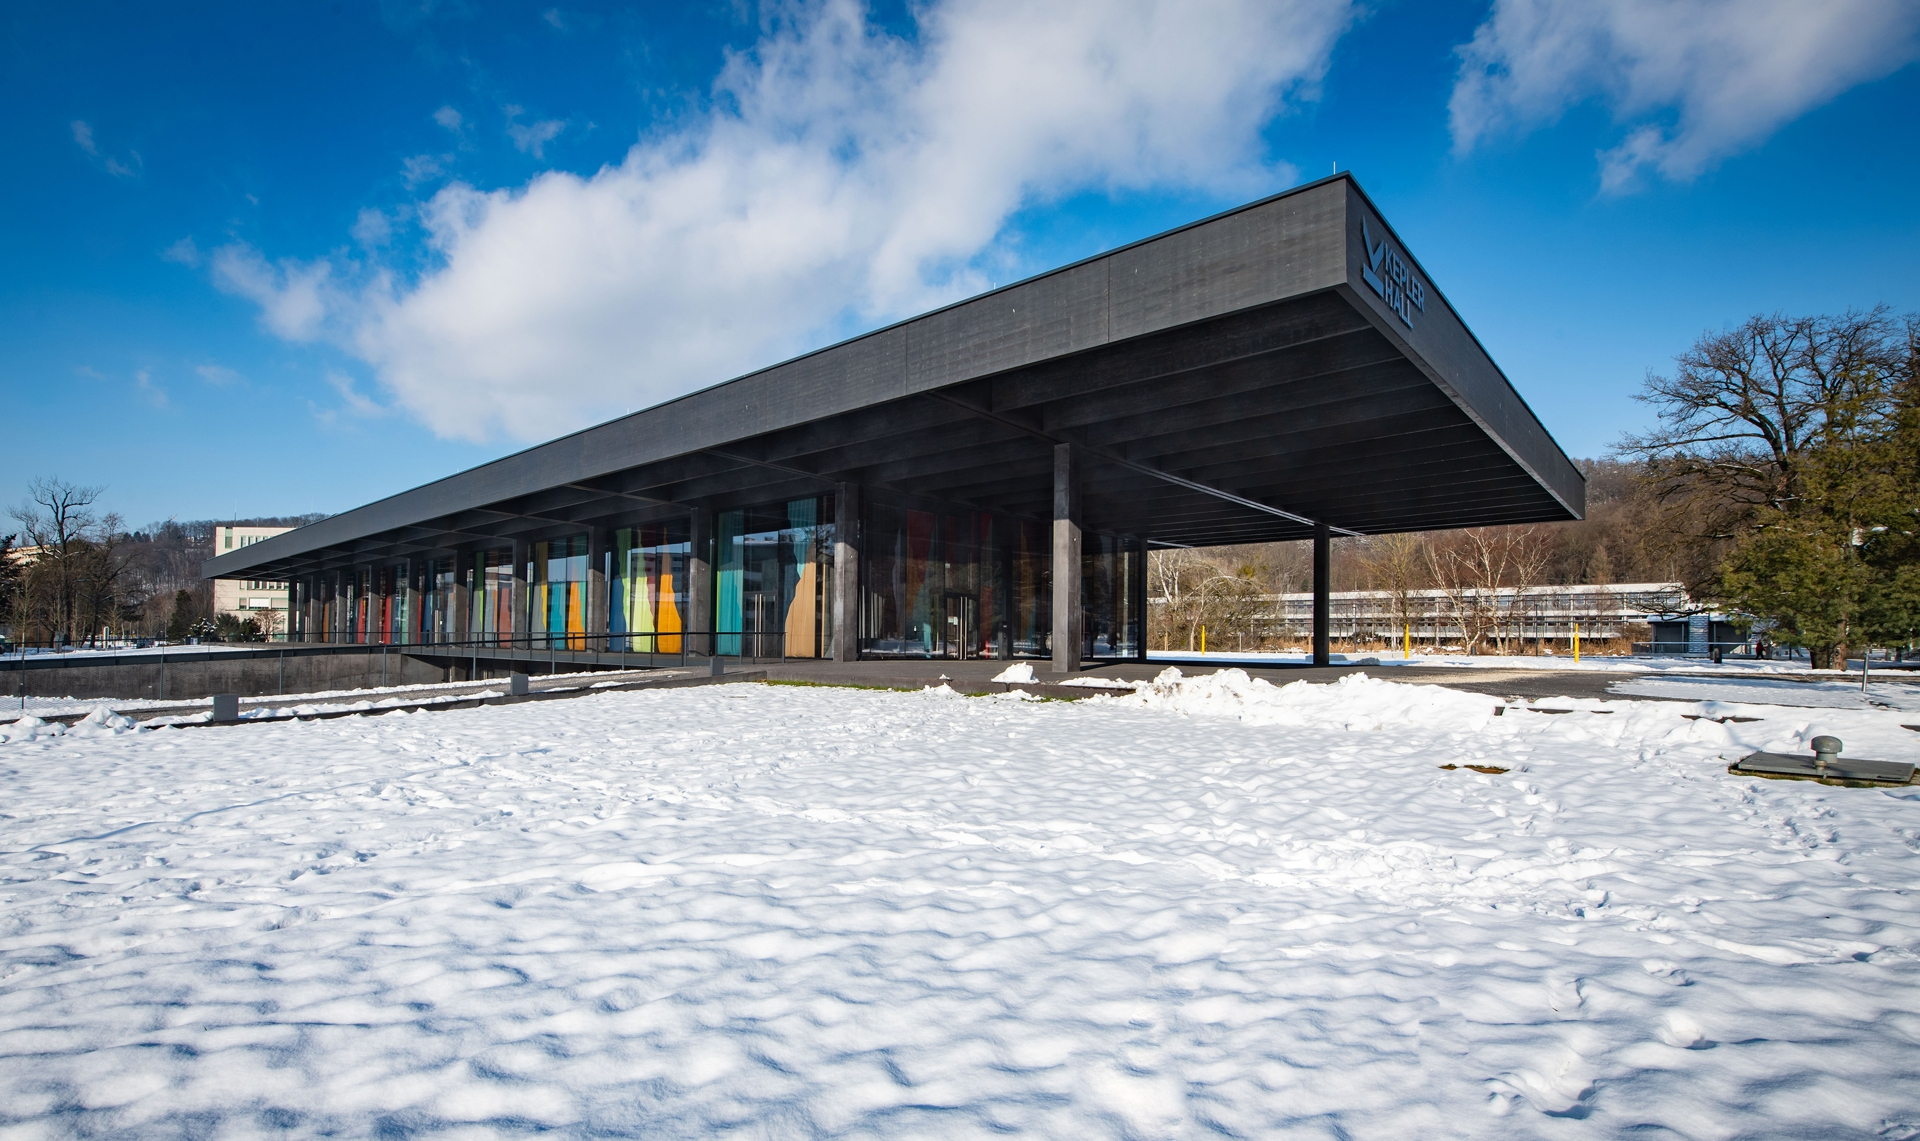
\includegraphics[width=\paperwidth]{images/jku_keplerhall_winter.jpg}}
\setbeamercolor{normal text}{fg=white}
\usebeamercolor[fg]{normal text}
\begin{frame}[plain]
\frametitle{Space for your frame title.}

Space for your frame body.
\end{frame}
\endgroup
\end{lstlisting}
\end{beamercolorbox}
\end{frame}
\endgroup


\begin{frame}[containsverbatim,plain]
\frametitle{Title Image Slide}

Use \verb|\imageframe[<mode options>]{<title>}{<subtitle>}{<graphic>}| to display a title image frame. That is a full screen image with a title sidebar.

\begin{lstlisting}[language={[LaTeX]TeX},numbers=none]
\imageframe{%
    This is an image frame.
}{%
    With a subtitle.
}{%
    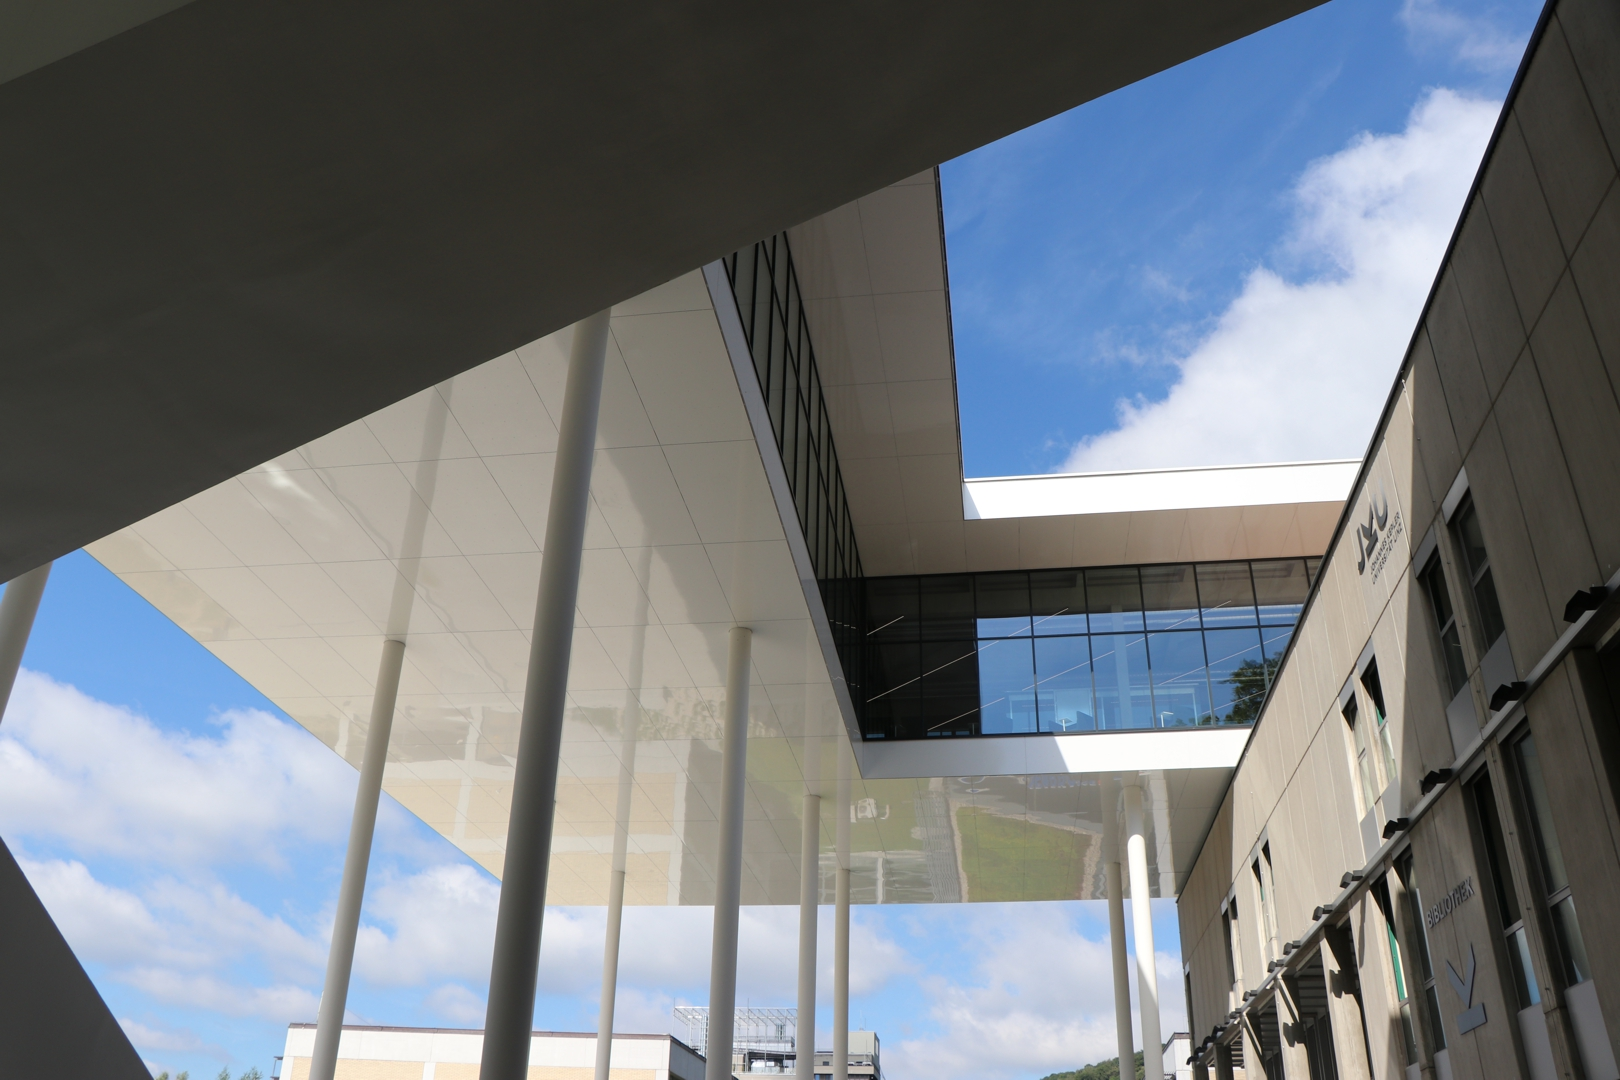
\includegraphics[height=\paperheight]{images/jku_learningcenter.jpg}
}
\end{lstlisting}

The optional argument ``\textverb{<mode options>}'' may be any of the color mode options that can be used for the \verb|\maketitle| command (see slide~\ref{advanced-title-slides}).
\end{frame}

\imageframe[dark]{%
    This is a title image frame.
}{%
    With a subtitle.
}{%
    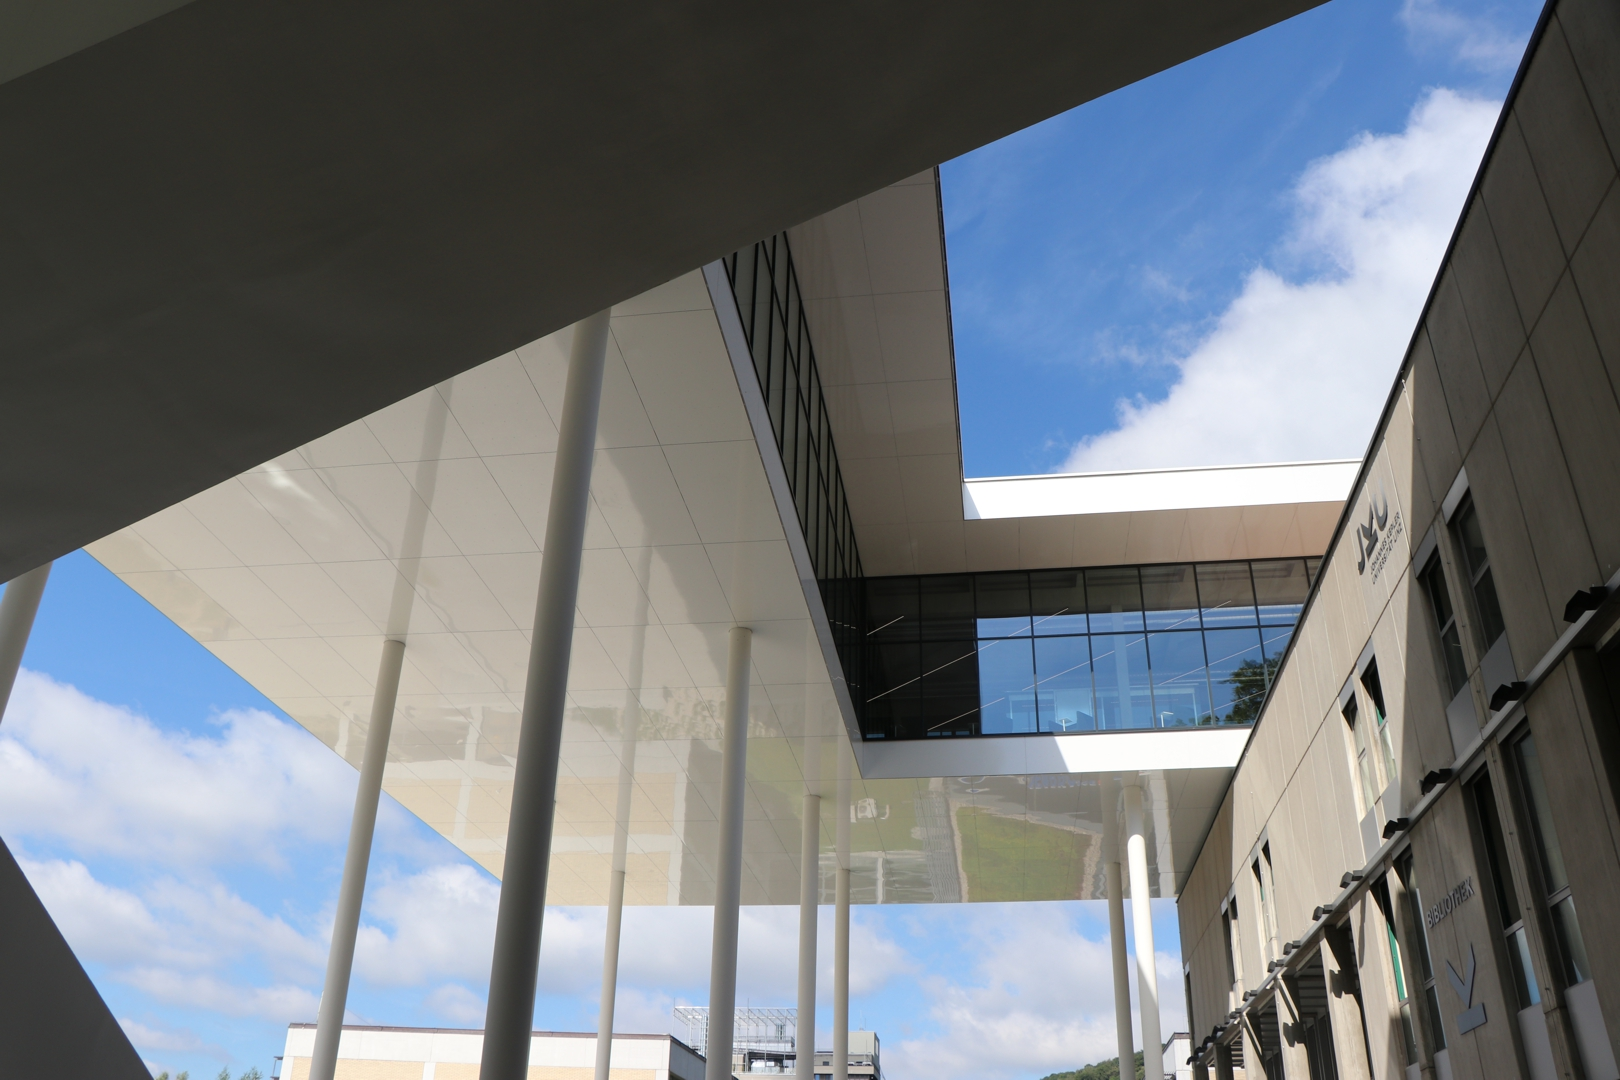
\includegraphics[height=\paperheight]{images/jku_learningcenter.jpg}
}

\imageframe[dark,MED]{%
    This is a title image frame.
}{%
    For the MED faculty.
}{%
    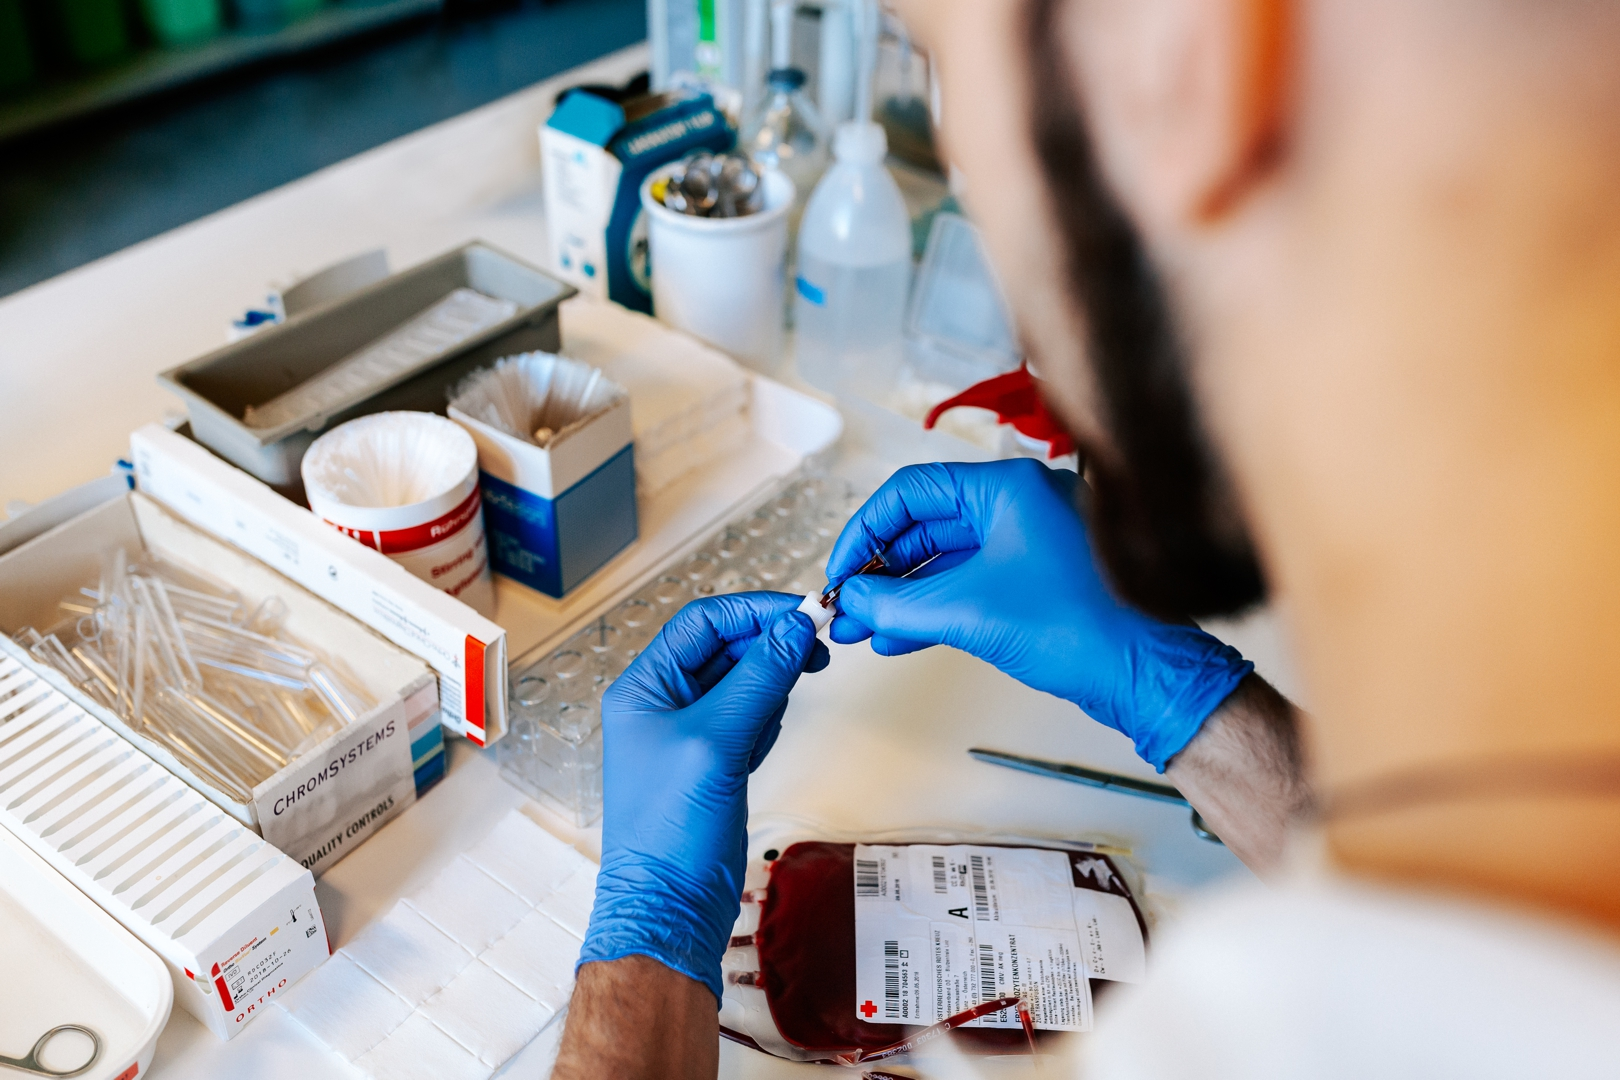
\includegraphics[height=\paperheight]{images/jku_med_image.jpg}
}


\begin{frame}[containsverbatim]
\frametitle{Logo Slides}

Use \verb|\jkulogo[<mode options>]| to display a logo slide. That is a slide with only the JKU logo centered on it. This slide is well suited as a final slide in your presentation.

Again, the optional argument ``\textverb{<mode options>}'' may be any of the color mode options that can be used for the \verb|\maketitle| command (see slide~\ref{advanced-title-slides}), e.g.
\begin{itemize}
\item \textverb{\string\jkulogo}
\item \textverb{\string\jkulogo[light]}
\item \textverb{\string\jkulogo[dark]}
\item \textverb{\string\jkulogo[SOWI,dark]}
\item \textverb{\string\jkulogo[gray]}
\item \textverb{\string\jkulogo[black]}
\end{itemize}
\end{frame}

\jkulogo
\jkulogo[light]
\jkulogo[dark]
\jkulogo[SOWI,dark]
\jkulogo[gray]
\jkulogo[black]


\begin{frame}[containsverbatim]
\frametitle{Switching Color Mode and Scheme}

Just like switching the color mode and scheme for a specific special slide, you can also switch the color mode for the remaining part of the presentation. This may be useful if you want to create a presentation with parts focusing on more than one faculty.

Use \verb|\setcolormode[<mode options>]| to change the color mode.
\end{frame}


\begin{frame}[containsverbatim,allowframebreaks]
\frametitle{Contact Information Slide}

Use \verb|\contactframe[<mode options>]{<name>}{<affiliation>}{<contact info>}{<ack>}| to display a contact information frame. 
\begin{lstlisting}[language={[LaTeX]TeX},numbers=none]
\contactframe{Johanna Kepler}{Institute of Networks and Security}{%
    \contactphone{+43 732 2468-XXXX}
    \contactmail{firstname.lastname@jku.at}
    \contactweb[https://www.jku.at/ins]{jku.at/ins}
}{%
    This work is funded by XYZ.
}
\end{lstlisting}
The optional argument ``\textverb{<mode options>}'' may be any of the color mode options that can be used for the \verb|\maketitle| command (see slide~\ref{advanced-title-slides}).

\framebreak
The contact info field may contain a combination of the following commands:
\begin{itemize}
\item \verb|\contactaddress{address}|: adds an address/place
\item \verb|\contactphone{number}|: adds a phone number
\item \verb|\contactfax{number}|: adds a fax number
\item \verb|\contactmail{e-mail address}|: adds an e-mail address
\item \verb|\contactweb[real url]{display url}|: adds a URL
\item \verb|\contactother[icon]{contact info}|: adds an arbitrary contact info entry, use \verb|\fa...| (from \verb|fontawesome5| package) as icons
\item \verb|\contactnewline|: adds an empty line
\end{itemize}
\end{frame}

\contactframe[dark]{%
    Johanna Kepler
}{%
    Institute of Networks and Security
}{%
    \contactphone{+43 732 2468-XXXX}
    \contactmail{firstname.lastname@jku.at}
    \contactweb[https://www.jku.at/ins]{jku.at/ins}
}{%
    This work is funded by XYZ.
}

\contactframe[light]{%
    Johanna Kepler
}{%
    Institute of Networks and Security
}{%
    \contactphone{+43 732 2468-XXXX}
    \contactmail{firstname.lastname@jku.at}
    \contactweb[https://www.jku.at/ins]{jku.at/ins}
}{%
    This work is funded by XYZ.
}






\section{General \LaTeX/Beamer Features}


\begin{frame}
\frametitle{Environments}

Standard \LaTeX-beamer defines several environments like
\begin{quote}
theorem, corollary, fact, lemma, problem, solution, definition, definitions, example, and examples.
\end{quote}

\begin{definition}[Monoid]
We call $(M,\circ)$ a \emph{monoid} if and only if
\begin{gather*}
\forall a,b,c\in M:\quad(a\circ b)\circ c = a\circ(b\circ c) \tag{associativity}\\
\exists e\in M \;\forall a\in M:\quad a\circ e = e\circ a= a \tag{neutral element}
\end{gather*}
\end{definition}
\end{frame}

\begin{frame}
\frametitle{Environments}

\begin{theorem}[Fundamental Theorem of \ldots]
Let $(M,+)$ be a monoid. Then \ldots
\end{theorem}

\begin{proof}
Let $M$ be an arbitrary set. We then show \ldots
\end{proof}

\begin{example}
Put an example here.
\end{example}
\end{frame}


\begin{frame}[fragile]
\frametitle{Self-defined Environments}

You also can define your own environments:
\begin{lstlisting}[language={[LaTeX]TeX},numbers=none]
\newtheorem{idea}[theorem]{Idea}

\begin{idea}[My own idea]
Here is a self-defined environment
\end{idea}

\theoremstyle{definition}
\newtheorem{defi}[theorem]{My Definition}

\begin{defi}
Test
\end{defi}
\end{lstlisting}
\end{frame}

\newtheorem{idea}[theorem]{Idea}
\theoremstyle{definition}
\newtheorem{defi}[theorem]{My Definition}
\theoremstyle{example}
\newtheorem{ex}[theorem]{My Example}

\begin{frame}[fragile]
\frametitle{Self-defined Environments}

\begin{idea}[My own idea]
Here is a self-defined environment
\end{idea}

\begin{defi}
Test
\end{defi}

\begin{ex}
Test
\end{ex}
\end{frame}


\begin{frame}[fragile]
\frametitle{Custom Blocks}
\begingroup
\setbeamercolor{block title}{fg=white,bg=jkuBlue}
\begin{block}{Blue block}
Using the theme colors to generate colored blocks.
\end{block}
\endgroup

\begin{lstlisting}[language={[LaTeX]TeX},numbers=none]
\begingroup
\setbeamercolor{block title}{fg=white,bg=jkuBlue}
\begin{block}{Blue block}
Use the theme colors to generate colorful blocks.
\end{block}
\endgroup
\end{lstlisting}
\end{frame}


\begin{otherlanguage}{ngerman}
\begin{frame}[fragile]
\frametitle{Language}
\begin{itemize}
\item Use the \textverb{otherlanguage} environment to temporarily change the document language in your presentation.
\item Changing the document language to \textverb{german} (or better \textverb{ngerman}) also changes the language in logos and the imprint on title pages and in footers.
\end{itemize}

\begin{lstlisting}[language={[LaTeX]TeX},numbers=none]
\begin{otherlanguage}{ngerman}

\end{otherlanguage}
\end{lstlisting}
\end{frame}
\end{otherlanguage}


\begin{frame}[label=handout]
\frametitle{Producing Handouts}

\begin{itemize}
\item You can generate a ``handout'' version of your presentation with the class option \textverb{handout}.
\item Section slides and logo slides will be suppressed.
\item Overlays will be flattened into single pages.
\item Slide numbering will still match the numbering in the non-handout version.
\end{itemize}
\end{frame}


\section{Ending the Presentation}

\begin{frame}
\frametitle{Thank You Thank You Thank You Thank You Thank You Thank You Thank You Thank You Thank You}

You see, btw., the slide title can run over several lines \ldots

\bigskip
\begin{alertblock}{Please \ldots}
\ldots\ refrain from putting an extra slide at the end saying ``\alert{Thank you for your attention}''. This is really annoying~\cite{schultz,karol}. You can say ``Thank you'' anyway, it need not be written. Instead, you can put a nice \textverb{\string\jkulogo} as the final slide!
\end{alertblock}

\end{frame}


\begin{frame}[allowframebreaks]{References}
%\setbeamerfont{bibliography item}{size={\footnotesize}}
%\AtNextBibliography{\footnotesize}
\printbibliography
\end{frame}


\begin{frame}
\frametitle{JKU Theme Information}

This a beamer theme for \href{https://www.jku.at/}{Johannes Kepler University Linz, Austria}.

\bigskip
\begin{exampleblock}{Want to report a bug? Want to request improvements?}
You are always welcome to suggest improvements via the official repository at \url{https://github.com/michaelroland/jku-templates-presentation-latex}.
\end{exampleblock}
\end{frame}


\jkulogo

\end{document}
\endinput
